\documentclass[12pt, a4paper]{article}

\usepackage[czech]{babel}
%\usepackage[IL2]{fontenc}
\usepackage[utf8]{inputenc}
\usepackage{enumitem}
\usepackage{parskip}
\usepackage{tocloft}
\usepackage{multicol}
\usepackage[hidelinks]{hyperref}
\usepackage{graphicx}
\usepackage{float}
\usepackage{listings}
\usepackage{xcolor}

% Define code style for C
\lstset{
    language=C,
    basicstyle=\ttfamily,
    keywordstyle=\color{blue},
    stringstyle=\color{red},
    commentstyle=\color{green},
    breaklines=true
    frame=shadowbox,
    numbers=left,
    numberstyle=\small,
    stepnumber=1,
    numbersep=5pt,
    showstringspaces=false,
    tabsize=4,
    captionpos=b,
}


\begin{document}

%Uvodni strana
\begin{titlepage}
    
\includegraphics[width=0.75\textwidth]{img/fav.png}
    \begin{center}
        
        
        \vspace{2cm}
        
        \Huge
        Semestrální práce KIV/UPS
        
        \vspace{1cm}
        
        \LARGE
        Úvod do počítačových sítí
        
        \vfill
        
        \vspace{0.5cm}
        
        \normalsize
        \raggedright
        Student:        Adam Míka \\
        Osobní číslo:   A22B0319P \\
        Email:          mikaa@students.zcu.cz \\
        Datum:          20. září 2024
        \vspace{0.2cm}
        
    \end{center}
\end{titlepage}

%tečky v obsahu
\renewcommand{\cftsecleader}{\cftdotfill{\cftdotsep}}
\renewcommand{\cftsubsecleader}{\cftdotfill{\cftdotsep}}
\renewcommand{\cftsubsubsecleader}{\cftdotfill{\cftdotsep}}

%obsah
\setcounter{page}{2}
\tableofcontents
\listoffigures
\lstlistoflistings
\begin{thebibliography}{99}
    \bibitem{image1ref} Zdroj Obrázku 1: \url{https://philipstel.wordpress.com/2010/08/04/dictionary-based-algorithm-lempel-ziv-welch/}
  \end{thebibliography}
\pagebreak


\section{Zadání}
\large
\textbf{Hlavní cíle:}
\normalsize
Zbytek zadání zde: \href{https://home.zcu.cz/~ublm/files/PozadavkyUPS.pdf}{\textcolor[RGB]{20,20,200}{\underline{\textit{PDF}}}}


\section{Analýza úlohy}

Cílem této práce je navrhnout a implementovat komunikační protokol pro multiplayerovou hru „Rock-Paper-Scissors“ (kámen, nůžky, papír) v předmětu KIV/UPS. Hra je navržena pro dva hráče, kteří soutěží proti sobě ve více kolech (standardně 10 kol). Hráči nezávisle na sobě volí jednu ze tří možností (kámen, nůžky, nebo papír) a server poté rozhodne o výsledku daného kola. Celkové skóre je aktualizováno po každém kole a po skončení všech kol je určen celkový vítěz.

\subsection{Popis protokolu}

Komunikační protokol je navržen tak, aby podporoval různé fáze hry a přechody mezi těmito fázemi. Diagram na obrázku \ref{fig:protocol} znázorňuje jednotlivé stavy protokolu a zprávy, které zajišťují přechody mezi těmito stavy.

\begin{figure}[H]
    \centering
    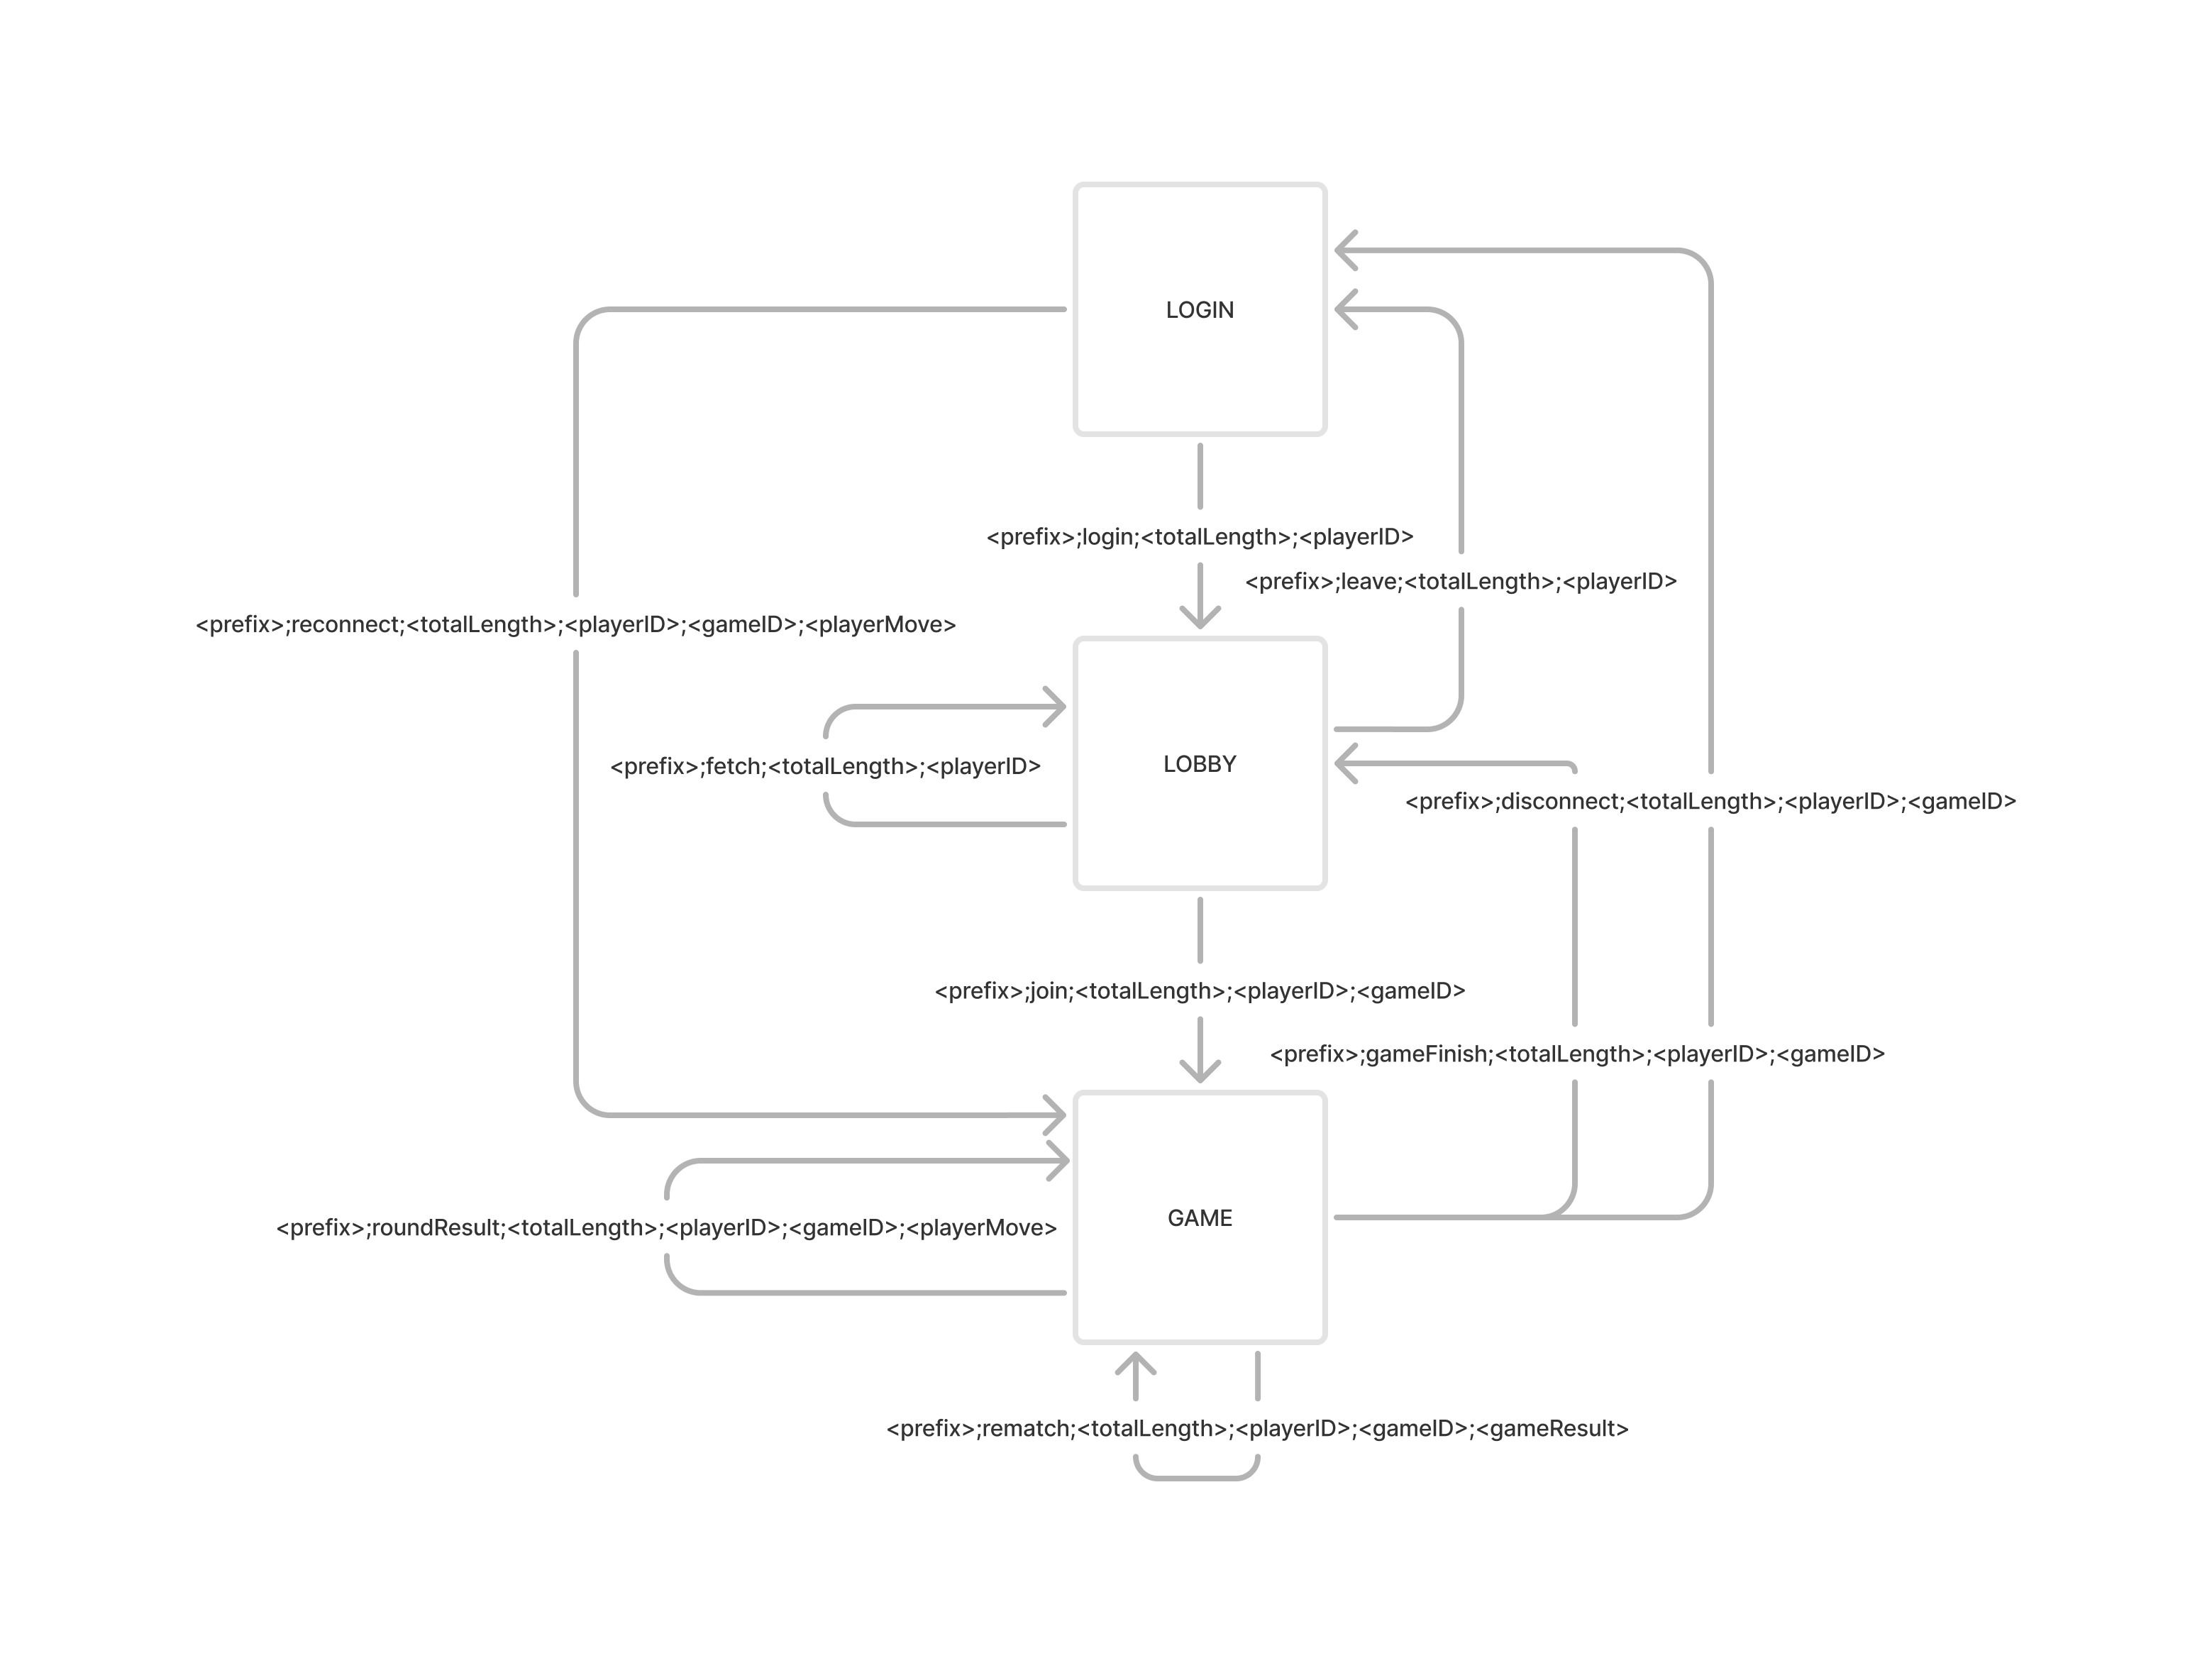
\includegraphics[width=0.8\textwidth]{img/protocol.png}
    \caption{Stavový diagram komunikačního protokolu pro hru Rock-Paper-Scissors}
    \label{fig:protocol}
\end{figure}

Diagram zahrnuje následující stavy a přechody:

\begin{itemize}
    \item \textbf{LOGIN}: Tento stav nastává při přihlášení hráče do systému. Hráč může odeslat zprávu pro přihlášení, opuštění nebo opětovné připojení k dříve přerušené hře. Příklady zpráv:
    \begin{itemize}
        \item \texttt{<prefix>;login;<totalLength>;<playerID>} – přihlášení hráče s identifikátorem \texttt{<playerID>}.
        \item \texttt{<prefix>;leave;<totalLength>;<playerID>} – opuštění lobby hráčem.
    \end{itemize}

    \item \textbf{LOBBY}: Po úspěšném přihlášení se hráč nachází v lobby, kde čeká na připojení dalších hráčů. Možné akce zahrnují připojení k existující hře nebo opuštění lobby. Příklady zpráv:
    \begin{itemize}
        \item \texttt{<prefix>;join;<totalLength>;<playerID>;<gameID>} – připojení hráče ke hře s identifikátorem \texttt{<gameID>}.
        \item \texttt{<prefix>;fetch;<totalLength>;<playerID>} – načtení aktuálních informací o lobby.
    \end{itemize}

    \item \textbf{GAME}: Jakmile je hra zahájena, hráči vstoupí do herního režimu, kde odesílají své tahy a server vyhodnocuje výsledky jednotlivých kol. Po ukončení hry je možné zaslat zprávu o jejím dokončení nebo požádat o odvetu. Příklady zpráv:
    \begin{itemize}
        \item \texttt{<prefix>;roundResult;<totalLength>;<playerID>;<gameID>;<playerMove>} – výsledek kola pro hráče.
        \item \texttt{<prefix>;gameFinish;<totalLength>;<playerID>;<gameID>} – ukončení hry.
        \item \texttt{<prefix>;rematch;<totalLength>;<playerID>;<gameID>;<gameResult>} – žádost o odvetu po skončení hry.
    \end{itemize}
    
    \item \textbf{DISCONNECT}: V kterémkoli stavu může dojít k odpojení hráče pomocí zprávy \texttt{<prefix>;disconnect;<totalLength>;<playerID>;<gameID>}, která signalizuje ukončení připojení.
\end{itemize}

Navržený protokol umožňuje efektivní komunikaci mezi klientem a serverem a podporuje různé přechody mezi stavy podle vývoje hry. Struktura zpráv zahrnuje předponu \texttt{<prefix>}, délku zprávy \texttt{<totalLength>}, identifikátor hráče \texttt{<playerID>} a další volitelné parametry, jako jsou \texttt{<gameID>} nebo \texttt{<playerMove>}.

Tento komunikační protokol zajišťuje spolehlivou výměnu dat mezi hráči a serverem a umožňuje flexibilní rozšíření o další funkce nebo herní módy.


\section{Ipmlementace}

\section{Uživatelská příručka}

\section{Závěr}

\end{document}
